\documentclass[tikz, border=1mm]{standalone}
\usepackage{tikz} 
\usetikzlibrary{arrows.meta}
\usepackage{pgfplots}

\pgfplotsset{compat=1.18}

\begin{document}

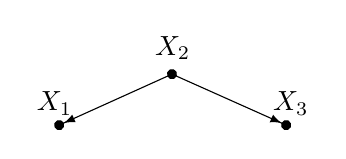
\begin{tikzpicture}

    % dag_bb1
    \node at (-1.5,0) {$X_{1}$};
    %\node at (0,0) {$X_{2}$}; 
    %\draw[black, fill=black] (-1.5,-0.3) circle(1.6pt);
    %\draw[black, fill=black] (0,-0.3) circle(1.6pt);

    % dag_bb2
    %\draw[{Circle}-{latex}{Circle}](-1.55,-0.3) to (0.05,-0.3); % X1 -> X2 (circle)
    
    % dag_bb3
    \node at (1.5,0) {$X_{3}$};
    %\draw[{Circle}-{latex}](-1.5,-0.3) to (0,-0.3); % X1 -> X2
    %\draw[{Circle}-{latex}{Circle}](0,-0.3) to (1.5,-0.3); % X2 -> X3
    
    % dag_bb4
    \node at (0,0.7) {$X_{2}$}; % top
    \draw[{Circle}-{latex}{Circle}](0.05,0.4) to (-1.5,-0.3); % X2 -> X1 (top)
    \draw[-{latex}{Circle}](0,0.37) to (1.5,-0.3); % X2 -> X3 (top)
    
    % dag_bb5
    %\node at (0,-1.2) {$X_{2}$}; % bottom
	%\draw[{Circle}-{latex}](-1.5,-0.3) to (0,-0.85); % X1 -> X2 (bottom)
    %\draw[{Circle}-{latex}{Circle}](1.5,-0.3) to (0,-0.9); % X3 -> X2 (bottom)
    
\end{tikzpicture}

\end{document}
